% Beamer slides: v8/v9 approach, results, low-confidence -> Suspect, DAC variant
% Compile: TEXINPUTS=./style: pdflatex slides_v8_v9.tex
\documentclass[aspectratio=169]{beamer}

% --- ORNL style (metropolis + ORNL branding assets) -----------------------
% Make sure pdflatex can find the .sty files in ./style and the assets in
% ./style/assets. If your local pdflatex doesn't pick the style folder up via
% \usepackage path, run with: TEXINPUTS=./style: pdflatex slides_v8_v9.tex
\makeatletter
\def\input@path{{style/}}
\makeatother

\usetheme{metropolis}
\usepackage{booktabs}
\usepackage{xcolor}
\usepackage{graphicx}
\usepackage{tikz}
\usepackage{url}
\graphicspath{{cases_v8_FINAL/}{predictions_v8_FINAL_full_train/}{style/assets/}}

% --- ORNL palette (approximate) -------------------------------------------
\definecolor{ornlGreen}{HTML}{007934}
\definecolor{ornlDark}{HTML}{1A1A1A}
\setbeamercolor{alerted text}{fg=ornlGreen}
\setbeamercolor{progress bar}{fg=ornlGreen, bg=ornlGreen!30}
\setbeamercolor{title separator}{fg=ornlGreen, bg=ornlGreen}
\setbeamercolor{progress bar in head/foot}{fg=ornlGreen, bg=ornlGreen!30}
\setbeamercolor{progress bar in section page}{fg=ornlGreen, bg=ornlGreen!30}
\setbeamercolor{frametitle}{fg=white, bg=ornlGreen}

% --- ORNL background frames -----------------------------------------------
% title_frame.png  -> background for the title slide
% slide_frame.png  -> background for every other slide
% ornl_logo.png    -> small ORNL logo (used by metropolis institute / title)
\newcommand{\ornltitlebg}{%
  \setbeamertemplate{background canvas}{%
    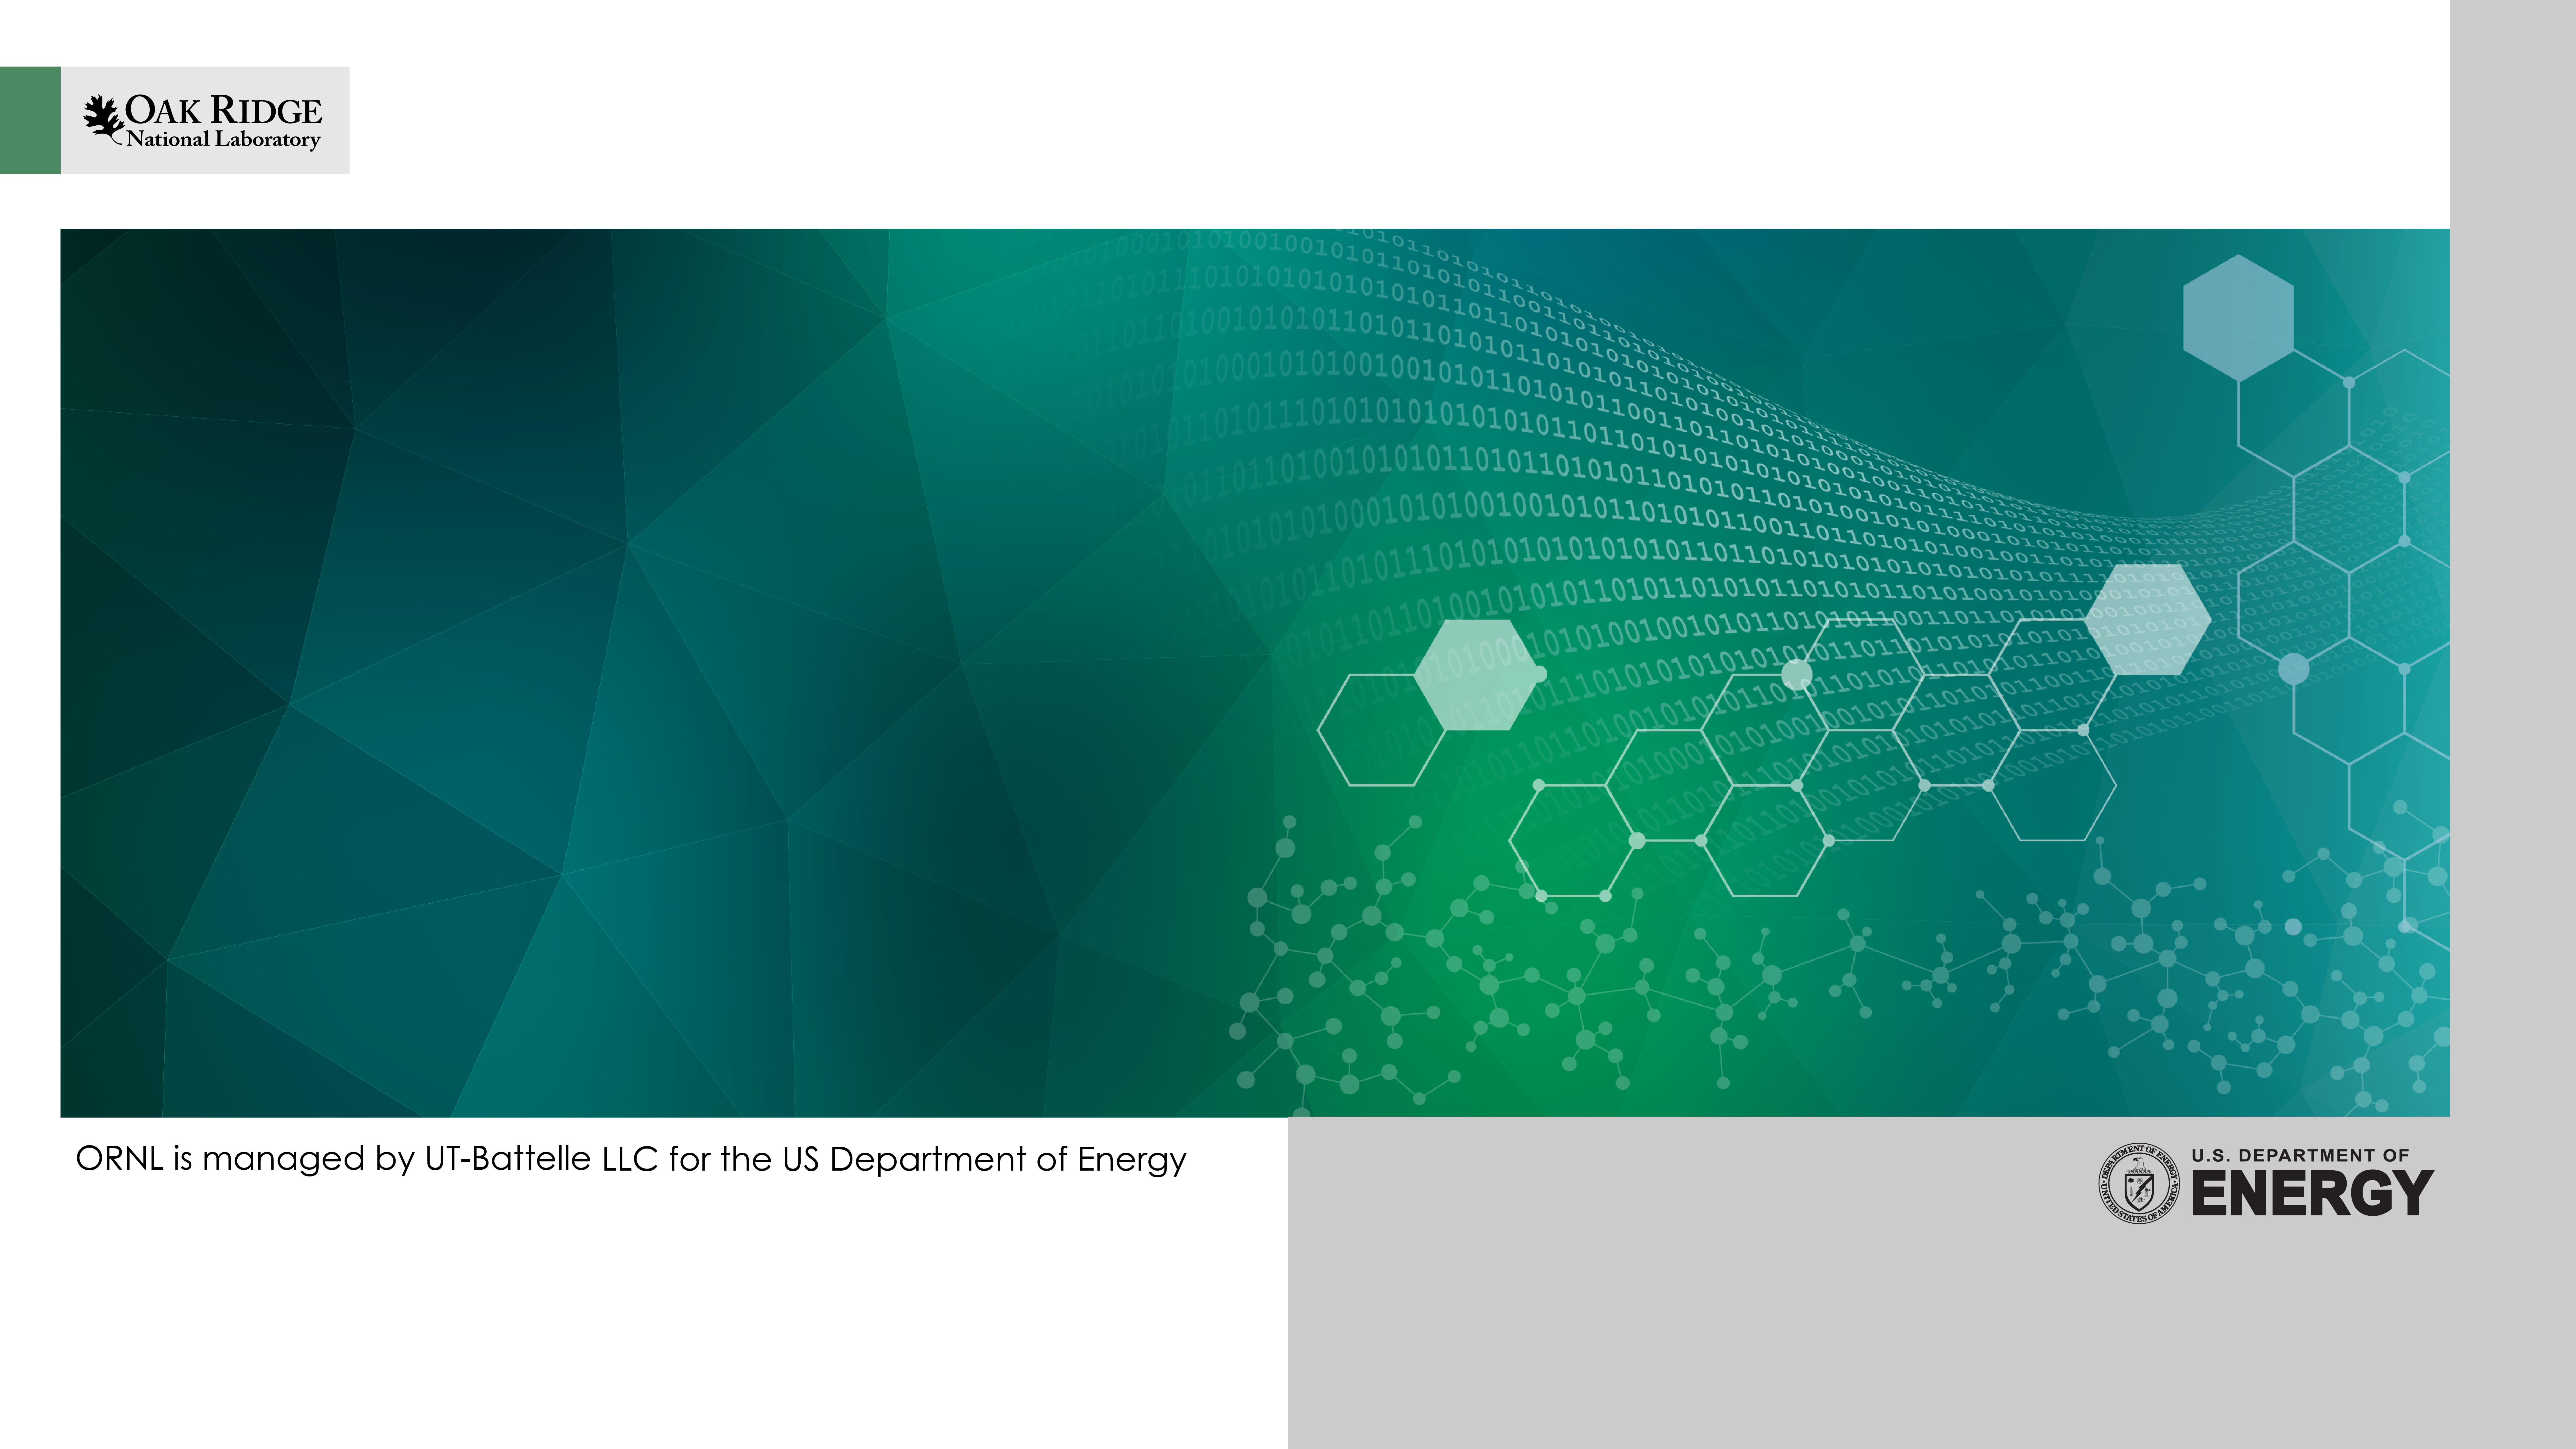
\includegraphics[width=\paperwidth,height=\paperheight,keepaspectratio=false]{title_frame.png}%
  }%
}
\newcommand{\ornlslidebg}{%
  \setbeamertemplate{background canvas}{%
    
\includegraphics[width=\paperwidth,height=\paperheight,keepaspectratio=false]{slide_frame.png}%
  }%
}

\title{Wind QC Classification: v8 \& v9 Pipeline}
\subtitle{From exploration to ablation to final models}
\date{\today}
\author{%
  Jose Tupayachi\inst{1} \and
  Kevin Birdwell\inst{1} \and
  John Ciolek\inst{2} \and
  Xiaoying Yu\inst{1} %
}
\institute{%
  \inst{1}Oak Ridge National Laboratory\par
  \inst{2}Los Alamos National Laboratory%
}
\titlegraphic{\hfill
\includegraphics[height=0.9cm]{ornl_logo.png}}

% --- Title-slide text in white (over dark title_frame.png background) --------
\setbeamercolor{title}{fg=white}
\setbeamercolor{subtitle}{fg=white}
\setbeamercolor{author}{fg=white}
\setbeamercolor{date}{fg=white}
\setbeamercolor{institute}{fg=white}

\begin{document}

% Title slide with the ORNL title-frame background
{%
  \ornltitlebg%
  \maketitle
}

% All subsequent frames use the ORNL slide-frame background
\ornlslidebg

% ======================================================================
\begin{frame}{Approach \& Methodology}
  \textbf{Goal.} 3-class wind-station QC classification (\textit{Good} / \textit{Bad} / \textit{Suspect})
  from QA plots of speed and direction time series.

  \medskip
  \textbf{Pipeline evolution.}
  \begin{enumerate}
    \tiny
    \item \alert{Initial exploration.} Visualised raw metadata, built pattern only PNGs
          (speed \& direction), profiled class balance and per-source skew.
          % (LANL vs.\ ORNL; Good : Bad : Suspect $\approx$ 3 : 3 : 2).
    \item \alert{Ablation study.} Swept backbones, fusion strategies, samplers,
          seeds, and pathways. Best configuration:
          \texttt{SwinV2-Large-192-22k} backbone, \texttt{concat} fusion,
          no weighted sampler.
    \item \alert{Final training (FULL\_TRAIN).} 15\% joint-stratified holdout
          , 30 epochs, early
          stopping with patience=10, best checkpoint kept.
  \end{enumerate}

  \medskip
  \textbf{v8 vs.\ v9.}
  \begin{itemize}
    \tiny
    \item \textbf{v8} - vision-only: SwinV2 features over speed \& direction QA images,
          fused (\texttt{concat}) into a 3-way classifier.
    \item \textbf{v9} - vision + LLM: adds Qwen3-VL captions $\rightarrow$
          1024-d Snowflake-Arctic-Embed2 embeddings cached per station,
          concatenated to SwinV2 features before the classifier.
  \end{itemize}
\end{frame}

% ======================================================================
\begin{frame}{Final Models, Results \& Inference}
  \textbf{15\% stratified holdout (60 stations) - joint by source $\times$ class.}

  \begin{center}
  \tiny
  \begin{tabular}{lcccc}
    \toprule
    Model & Val F1 & Suspect F1 & Accuracy & Best epoch \\
    \midrule
    v8 (vision)        & \textbf{0.7690} & 0.6897 & 0.767 & 10 \\
    v9 (vision + LLM)  & 0.7593 & 0.6400 & 0.767 & 6 \\
    % \midrule
    % LANL$\rightarrow$ORNL v8 & 0.5073 & - & - & - \\
    % LANL$\rightarrow$ORNL v9 & \textbf{0.5511} & - & - & - \\
    \bottomrule
  \end{tabular}
  \end{center}

  \medskip
  \textbf{Take-aways.}
  \begin{itemize}
    \tiny
    \item In-domain: v8 and v9 are statistically tied; vision alone is strong.
    \item \textbf{Cross-domain (LANL$\rightarrow$ORNL): the LLM pathway helps}
          ($+4.4$ F1), suggesting captions encode domain-invariant signal.
    \item Hardest class is \textit{Suspect} - many predictions live near the
          decision boundary ($p_{\max}\!\approx\!0.4$-$0.55$).
  \end{itemize}

  \textbf{Inference workflow.} Run the saved checkpoint on unlabeled ORNL,
  then \emph{flag low-confidence predictions as Suspect} for human review
  rather than committing to Good/Bad.
\end{frame}

% ======================================================================
\begin{frame}{Confidence-Aware ``Suspect'' Routing}
  \textbf{Inference-time rule.} For each station with
  softmax probabilities $p_g, p_b, p_s$:
  \[
    \hat{y} =
    \begin{cases}
      \texttt{Suspect} & \text{if } \max(p_g,p_b,p_s) < \tau
                          \;\;\text{or}\;\; |p_g-p_b| < \delta\\
      \arg\max_c p_c   & \text{otherwise}
    \end{cases}
  \]
  Defaults: $\tau=0.55$, $\delta=0.10$. Tune $\tau$ on the holdout to maximise
  Suspect recall at a fixed Good/Bad precision floor.

  \medskip
  \textbf{Adding this into training?} Yes - two options:
  \begin{itemize}
    \tiny
    % \item \alert{Soft labels / label smoothing on Suspect.} Train
    %       \textit{Suspect} as a mixture
    %       $(0.15, 0.15, 0.70)$ so the model learns it as ``ambiguous'',
    %       not a hard third class.
    \item \alert{Confidence-penalty / abstention loss. DAC} Add an \emph{Abstain}
          head $a\in[0,1]$ trained with the Deep-Abstaining-Classifier loss:
          \[
            \mathcal{L} = -(1-a)\log p_y - \alpha\log(1-a),
          \]
          which lets the model route uncertain samples into \textit{Suspect}
          automatically. $\alpha$ controls how often the model is allowed
          to abstain.
    \item \alert{Evidential / Dirichlet head.} Replace softmax with a Dirichlet
          output; map low total evidence $\rightarrow$ \textit{Suspect}.
  \end{itemize}

  \textbf{Recommendation.} v8 + threshold rule; + More control.
\end{frame}

% ======================================================================
\begin{frame}{v8/v9 + DAC: Training-Time Abstention}
  \textbf{What changed.}:
  \begin{itemize}
    \tiny
    \item \texttt{multi\_model\_trainingv8\_new\_dac.py} \;$\rightarrow$\;
          \texttt{model\_outputs\_v8\_FINAL\_full\_train\_DAC/}
    \item \texttt{multi\_model\_trainingv9\_new\_dac.py} \;$\rightarrow$\;
          \texttt{model\_outputs\_v9\_FINAL\_full\_train\_DAC/}
    \item Launchers: \texttt{run\_v8\_full\_train\_final\_dac.sh},
          \texttt{run\_v9\_full\_train\_final\_dac.sh}
  \end{itemize}

  \medskip
  \textbf{Architecture diff.} Classifier head outputs $K\!+\!1=4$ logits.
  The extra logit is the \emph{abstain} score $a=\sigma(\text{logit}_{K+1})$.
  Loss:
  \[
    \mathcal{L}_{\text{DAC}} \;=\; -(1-a)\log p_y \;-\; \alpha\log(1-a)
  \]
  At eval/inference the abstain mask is folded into the Suspect column,
  preserving the suspect class:
  % \[\tiny
  %   \tilde{p} = (1-a)\cdot\text{softmax}(\text{logits}_{1:K}),\qquad
  %   \tilde{p}_{\text{Suspect}} \mathrel{+}= a
  % \]

  % \medskip
  % \textbf{Why this should help.}
  % \begin{itemize}
  %   \item Model itself learns when to say ``I don't know'' instead of being
  %         forced into Good/Bad on hard inputs.
  %   \item Single hyperparameter $\alpha$ (env \texttt{DAC\_ALPHA}, default 1.0)
  %         controls abstention rate; sweep $\alpha\!\in\!\{0.5, 1.0, 2.0\}$
  %         on the same 15\% holdout and pick best Suspect F1.
  %   \item No change to data, splits, or any other hparam $\Rightarrow$ direct,
  %         honest comparison vs.\ the original v8/v9 FINAL runs.
  % \end{itemize}
\end{frame}

% ======================================================================
%  v8 FINAL inference deck (continuation)
% ======================================================================

% % ======================================================================
% \begin{frame}{Pipeline \& Approach Selection}
%   \textbf{Phase 1 - Exploration.}
%   \begin{itemize}
%     \item Inspected raw MesoWest CSVs (LANL + ORNL); built QA-style PNGs
%           for wind speed and direction time series.
%     \item Profiled class skew (Good : Bad : Suspect $\approx$ 3 : 3 : 2)
%           and per-source distribution differences (LANL vs.\ ORNL).
%     \item Tested one-pathway baselines (vision, time-series, gap-detection,
%           LLM caption embeddings) to confirm vision is the dominant signal.
%   \end{itemize}

%   \textbf{Phase 2 - Ablation study.}
%   \begin{itemize}
%     \item Swept 9 model versions (v1-v9) over backbones, fusion strategies,
%           weighted samplers, focal-loss variants, and seeds.
%     \item Evaluated each via 5-fold cross-validation; ranked by macro-F1.
%     \item Winner: \textbf{v8 + SwinV2-Large-192-22k}, fusion=\texttt{concat},
%           no weighted sampler, SEED=42, default loss.
%   \end{itemize}

%   \textbf{Phase 3 - Final training.}
%   \begin{itemize}
%     \item Single 85/15 \emph{joint stratified} split (source $\times$ class
%           $\rightarrow$ 6 cells, 334 train / 60 test).
%     \item 30 epochs, early stopping with patience=10, best checkpoint kept.
%     \item Inference on the 2{,}196 unlabeled ORNL stations $\rightarrow$ CSV/XLSX.
%   \end{itemize}
% \end{frame}

% ======================================================================
\begin{frame}{Architecture, Hyperparameters \& Performance}
  \textbf{v8 architecture.}
  \begin{itemize}
    \tiny
    \item \textbf{Vision backbone:} SwinV2-Large patch-4 window-12, 192px,
          22k-class pretraining. Two parallel passes - one for the
          \emph{speed} QA image, one for \emph{direction}.
    \item \textbf{1D-CNN time-series pathway} on the raw resampled signal.
    \item \textbf{Gap-detection pathway} (per-image missing-data score).
    \item \textbf{Concat fusion} $\rightarrow$ 2-layer MLP $\rightarrow$ softmax over
          \{Good, Bad, Suspect\}.
  \end{itemize}

  \textbf{Best ALL hyperparameters (selected by ablation macro-F1).}
  \begin{center}
  \tiny
  \begin{tabular}{lc}
    \toprule
    Setting & Value \\
    \midrule
    Backbone / fusion & SwinV2-Large-192-22k / \texttt{concat} \\
    Optimizer / LR / WD & AdamW / 2e-5 / 0.01 \\
    Batch size / Epochs & 4 / 30 (early-stop patience=10) \\
    Sampler / Loss & shuffle / CrossEntropy (focal disabled) \\
    Seed / Holdout & 42 / 15\% joint-stratified \\
    \bottomrule
  \end{tabular}
  \end{center}

  
\end{frame}



\begin{frame}
  \textbf{Held-out performance (60 stations).}
  \begin{itemize}

    \item Macro-F1 = \textbf{0.7690}; Accuracy = 0.7667
    \item Per-class F1: Good 0.7547 \;|\; Bad \textbf{0.8421} \;|\; Suspect 0.6897
    \item Best epoch = 10 (early-stop fired at 20)
  \end{itemize}

\end{frame}

% ======================================================================
\begin{frame}{v8 Confusion Matrix \& Pathway Importance}
  \begin{columns}[T]
    \begin{column}{0.50\textwidth}
      \centering
      \includegraphics[width=\linewidth,keepaspectratio]{confusion_matrix_v8.png}
    \end{column}
    \begin{column}{0.50\textwidth}
      \centering
      \includegraphics[width=\linewidth,keepaspectratio]{pathway_importance_by_class.png}
    \end{column}
  \end{columns}
  \begin{itemize}
    \tiny
    \item \textbf{Left:} Confusion matrix on the 60-station holdout (Acc 0.767, F1 0.769).
          Main confusion: Good$\leftrightarrow$Suspect (3+5 off-diagonal).
    \item \textbf{Right:} Average attention weight per pathway per class.
          Vision dominates for \textit{Good} (0.38); TimeSeries and GapDetection
          contribute more evenly for \textit{Bad} and \textit{Suspect}.
  \end{itemize}
\end{frame}

% ======================================================================
\begin{frame}{Inference Output \& What the CSV Means}
  \textbf{Files} ([predictions\_v8\_FINAL\_full\_train/]):
  \begin{itemize}
    \item \texttt{ornl\_unlabeled\_predictions.csv}, \texttt{.xlsx} (2 sheets)
    \item \texttt{selection.json} - traceability: checkpoint path, hparams, n\_stations
  \end{itemize}

  \textbf{Schema.}
  \begin{center}\small
  \begin{tabular}{ll}
    \toprule
    Column & Meaning \\
    \midrule
    \texttt{Station}      & MesoWest station ID (ORNL) \\
    \texttt{Category}     & Predicted class: Good / Bad / Suspect (argmax) \\
    \texttt{Reason}       & String - model, fusion, run, checkpoint \\
    \texttt{Source}       & ORNL (all rows) \\
    \texttt{P(Good)}      & Softmax probability for Good \\
    \texttt{P(Bad)}       & Softmax probability for Bad \\
    \texttt{P(Suspect)}   & Softmax probability for Suspect \\
    \texttt{confidence}   & $\max(P_g, P_b, P_s)$ - routing signal \\
    \bottomrule
  \end{tabular}
  \end{center}


\end{frame}


















\begin{frame}

  \textbf{Run summary (2{,}196 stations, 0 failures).}
  \begin{itemize}
    \item Distribution: \textbf{Good 706 \;|\; Bad 1{,}055 \;|\; Suspect 435}
    \item Mean confidence \textbf{0.904} (min 0.343, max 0.997)
  \end{itemize}
\end{frame}

% ======================================================================
%  Post-processed (4-class) case studies
% ======================================================================
\begin{frame}{Post-processed Distribution (4 classes)}
  \textbf{Confidence-aware reclassification} ($\tau\!=\!0.85$, $\delta\!=\!0.20$):
  any row whose top-1 probability $<\!0.85$ \emph{or} margin to runner-up $<\!0.20$ is
  routed to the new \alert{Suspect\_postprocess} class.

  \begin{center}
  \tiny
  \begin{tabular}{lcc}
    \toprule
    Class & Count & Share \\
    \midrule
    Bad                  & 867 & 39.5\% \\
    Good                 & 543 & 24.7\% \\
    Suspect              & 336 & 15.3\% \\
    \alert{Suspect\_postprocess} & \textbf{450} & \textbf{20.5\%} \\
    \midrule
    Total                & 2{,}196 & 100.0\% \\
    \bottomrule
  \end{tabular}
  \end{center}

  \medskip
  \textbf{Take-away.} 20.5\% of stations were originally argmax-classified as Good or Bad
  but lacked the confidence (or margin) to be trusted; they are now flagged
  for human review under the new label.
\end{frame}

\begin{frame}{Post-process Cases — Predicted \textit{Good} (543 stations)}
  \begin{columns}[T]
    \begin{column}{0.50\textwidth}
      \centering
      \includegraphics[height=0.78\textheight,keepaspectratio]{cases_pp_Good.png}
    \end{column}
    \begin{column}{0.50\textwidth}
      \textbf{Examples by confidence level.}
      \begin{itemize}
        \tiny
        \item \textbf{Extreme high} ($P{=}0.99$): \texttt{ASOS-AWOS\_KEKY}.
        \item \textbf{Average} ($P{=}0.97$): CWOP \texttt{C2722}.
        \item \textbf{Borderline} ($P{=}0.85$): CWOP \texttt{AT066} —
              just barely cleared $\tau{=}0.85$; runner-up $P(\text{Suspect})=0.12$.
      \end{itemize}
      \medskip
      All retained Good rows now satisfy $P(\text{Good})\!\geq\!0.85$ and a
      $\geq\!0.20$ margin over the next class.
    \end{column}
  \end{columns}
\end{frame}

\begin{frame}{Post-process Cases — Predicted \textit{Bad} (867 stations)}
  \begin{columns}[T]
    \begin{column}{0.50\textwidth}
      \centering
      \includegraphics[height=0.78\textheight,keepaspectratio]{cases_pp_Bad.png}
    \end{column}
    \begin{column}{0.50\textwidth}
      \textbf{Examples by confidence level.}
      \begin{itemize}
        \tiny
        \item \textbf{Extreme high} ($P{=}1.00$): \texttt{SCDOT\_SC010} —
              spiky speed + banded direction (instrument fault).
        \item \textbf{Average} ($P{=}0.98$): \texttt{IFLOWS\_ERHK2} — flat-line.
        \item \textbf{Borderline} ($P{=}0.85$): CWOP \texttt{D0777} —
              $P(\text{Good})=0.13$, just clears the floor.
      \end{itemize}
      \medskip
      Flat-line and spike modes still dominate; only ambiguous Bad rows are
      removed by the rule.
    \end{column}
  \end{columns}
\end{frame}

\begin{frame}{Post-process Cases — Predicted \textit{Suspect} (336 stations)}
  \begin{columns}[T]
    \begin{column}{0.50\textwidth}
      \centering
      \includegraphics[height=0.78\textheight,keepaspectratio]{cases_pp_Suspect.png}
    \end{column}
    \begin{column}{0.50\textwidth}
      \textbf{Examples by confidence level.}
      \begin{itemize}
        \tiny
        \item \textbf{Extreme high} ($P{=}1.00$): \texttt{RAWS\_CHKN7} —
              direction stuck on one heading.
        \item \textbf{Average} ($P{=}0.98$): \texttt{KYMN\_WKULUSA}.
        \item \textbf{Borderline} ($P{=}0.85$): CWOP \texttt{E3156} —
              clearly Suspect by argmax, but only just above the floor.
      \end{itemize}
      \medskip
      Original \textit{Suspect} predictions kept here are model-asserted with
      $P(\text{Suspect})\!\geq\!0.85$.
    \end{column}
  \end{columns}
\end{frame}

\begin{frame}{Post-process Cases — \alert{Suspect\_postprocess} (450 stations)}
  \begin{columns}[T]
    \begin{column}{0.50\textwidth}
      \centering
      \includegraphics[height=0.78\textheight,keepaspectratio]{cases_pp_Suspect_postprocess.png}
    \end{column}
    \begin{column}{0.50\textwidth}
      \textbf{The new ``must-review'' bucket.}
      \begin{itemize}
        \tiny
        \item \textbf{Extreme high} ($P{=}0.85$): CWOP \texttt{F7113} —
              originally Suspect, but $P{<}0.85$ failed by a hair.
        \item \textbf{Average} ($P{=}0.69$): CWOP \texttt{D3823} —
              originally Good with $P(\text{Good})=0.69$, $P(\text{Bad})=0.21$.
        \item \textbf{Borderline} ($P{=}0.34$): \texttt{GADOT\_GA303} —
              \emph{near-uniform} 3-way split (margin $0.001$); the model is
              effectively guessing.
      \end{itemize}
      \medskip
      Every row here was an original argmax that failed either the
      confidence floor ($\tau{=}0.85$) or the margin floor ($\delta{=}0.20$).
    \end{column}
  \end{columns}
\end{frame}

% ======================================================================
\begin{frame}{Acknowledgements}
  \small
  This work was supported by the
  \textbf{Nuclear Safety Research and Development (NSR\&D)} program,
  the \textbf{National Nuclear Security Administration (NNSA)},
  the \textbf{Office of Environment, Health, Safety, and Security (EHSS)},
  and the \textbf{U.S.\ Department of Energy (DOE)}
  (DOI: 10.13039/100000015).

  \medskip
  \tiny
  This manuscript has been authored by UT-Battelle, LLC, with the U.S.\
  DOE under Contract DE-AC05-00OR22725. The U.S.\ government retains and
  the publisher, by accepting the article for publication, acknowledges
  that the U.S.\ government retains a nonexclusive, paid-up, irrevocable,
  worldwide license to publish or reproduce the published form of this
  manuscript, or allow others to do so, for U.S.\ government purposes.
  DOE will provide public access to these results of federally sponsored
  research in accordance with the DOE Public Access Plan
  (\url{https://www.energy.gov/doe-public-access-plan}).
\end{frame}

\end{document}
